\documentclass[10pt,a4paper]{article}
\usepackage{tocloft}
\usepackage{commons/course}  % همین کافیه؛ listings و xcolor داخلشه
\usepackage{booktabs}

% Define colors for syntax highlighting
\definecolor{keywordstyle}{rgb}{0.0, 0.4, 0.8} % A bluer shade
\definecolor{stringstyle}{rgb}{0.9, 0.17, 0.31} % amaranth
\definecolor{commentstyle}{rgb}{0.1, 0.6, 0.2} % green
\definecolor{numberstyle}{rgb}{0.4, 0.4, 0.4} % gray
\definecolor{backgroundcolor}{rgb}{0.94, 0.97, 1.0} % aliceblue

% Define the Python-like language for syntax highlighting
\lstdefinelanguage{PythonLike}{
	morekeywords={mov, add, sub, cmp, jmp , lw , addi,sw,bne},
	sensitive=false,
	morecomment=[l]{;},
	morestring=[b]",
}

% Set the style for Python-like code
\lstset{
	language=PythonLike,
	basicstyle=\ttfamily\small,
	keywordstyle=\color{keywordstyle},
	stringstyle=\color{stringstyle},
	commentstyle=\color{commentstyle},
	numbers=left,
	numberstyle=\tiny\color{numberstyle},
	stepnumber=1,
	numbersep=5pt,
	keepspaces=true,
	tabsize=4,
	showspaces=false,
	showstringspaces=false,
	showtabs=false,
	breaklines=true,
	breakatwhitespace=false,
	frame=single,
	backgroundcolor=\color{backgroundcolor},
}

\newlistof{listofproblems}{lop}{\normalsize فهرست مسائل}
\newcommand{\addproblem}[1]{\addcontentsline{lop}{listofproblems}{\protect\numberline{}#1}}


\begin{document}


\سربرگ{آزمایش سوم}{ضرب‌کننده ممیز ثابت}{معین آعلی - ثمین اکبری}{استاد: دکتر حمید سربازی آزاد}

\subsubsection*{خلاصه}

در این آزمایش یک ضرب‌کننده‌ی دودویی ۴×۴ به روش \lr{Shift \& Add} در نرم‌افزار \lr{Logisim} طراحی و پیاده‌سازی شده است. مدار به‌صورت ترتیبی کار می‌کند و کاملا از تراشه‌های سری ۷۴ کتابخانه‌ی \lr{TTL} ساخته شده: \lr{7408} برای گیت‌های \lr{AND}، \lr{74283} برای جمع ۴ بیتی، دو عدد \lr{74194} به‌عنوان ثبات‌های \lr{ACC} و \lr{Q}، \lr{74161} برای شمارش چهار سیکل، و \lr{7404} برای ساخت سیگنال‌های کنترلی. مدار اصلی (\lr{multiplier}) طراحی هسته است و مدار \lr{main} همان هسته را با یک قطعه‌ی \lr{Clock} برای دمو می‌پیچد.



\subsubsection*{بلوک دیاگرام ضرب‌کننده}
\begin{figure}[h]
  \centering
  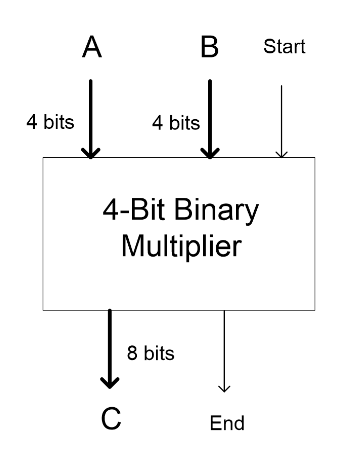
\includegraphics[width=0.3\textwidth]{figs/block.png}
\end{figure}


\subsubsection*{هدف آزمایش}

هدف از این آزمایش، طراحی و پیاده‌سازی یک ضرب‌کننده‌ی دودویی چهاربیتی به روش \lr{shift \& add} است. برخلاف ضرب‌کننده‌ی ترکیبی که همه‌ی حاصل‌ضرب‌های جزئی را یک‌جا جمع می‌کند، این مدار عملیات را در چند سیکل ساعت انجام می‌دهد و با سیگنال‌های \lr{Start}/\lr{End} شروع و پایان کار را اعلام می‌کند. اهداف مشخص این آزمایش عبارت‌اند از:

\begin{itemize}
  \item آشنایی عملی با الگوریتم ضرب ترتیبی \lr{Shift \& Add}.
  \item پیاده‌سازی مدار با تراشه‌های استاندارد \lr{TTL} سری ۷۴ (بدون گیت مجزا خارج از بسته‌ها).
  \item طراحی واحد کنترل با استفاده از پین‌های مد ثبات \lr{74194} و شمارنده‌ی \lr{74161}.
  \item بررسی صحت عملکرد با بردارهای تست ترتیبی، از جمله پوشش کامل ۲۵۶ ضرب ممکن.
\end{itemize}


\subsubsection*{رابط مدار}

\begin{center}
\begin{tabular}{@{}llll@{}}
\toprule
\textbf{سیگنال} & \textbf{جهت} & \textbf{پهنا} & \textbf{توضیح} \\
\midrule
\lr{A} & ورودی & ۴ & مضروب \\
\lr{B} & ورودی & ۴ & مضروب‌فیه \\
\lr{start} & ورودی & ۱ & سطحی؛ برای مقداردهی اولیه فعال می‌شود \\
\lr{clk} & ورودی & ۱ & لبه‌ی بالارونده \\
\lr{C} & خروجی & ۸ & حاصل‌ضرب \\
\lr{end} & خروجی & ۱ & با معتبرشدن \lr{C} فعال می‌شود \\
\bottomrule
\end{tabular}
\end{center}


\subsubsection*{الگوریتم \lr{Shift \& Add}}

ثبات‌ها: $\mathrm{ACC}[3:0]$ (انباره)، $\mathrm{Q}[3:0]$ (مضروب‌فیه)، و $M[3:0]=A$ (مضروب، روی پین‌های ورودی ثابت).

هر سیکل {جمع و شیفت را با هم} در یک لبه‌ی ساعت انجام می‌دهد:
\[
\begin{aligned}
\{\mathrm{Cout},\, S[3:0]\} &= \mathrm{ACC} + (Q_0\,?\, M : 0) \\
\mathrm{ACC} &\leftarrow \{\mathrm{Cout},\, S_3,\, S_2,\, S_1\} \\
Q &\leftarrow \{S_0,\, Q_3,\, Q_2,\, Q_1\}
\end{aligned}
\]

پس از ۴ تکرار: $C[7:4]=\mathrm{ACC}$ و $C[3:0]=Q$.

ردیابی دستی برای $A=3$ و $B=3$:

\begin{LTR}
\begin{center}
\begin{tabular}{@{}ccccc@{}}
\toprule
cycle & ACC & Q & Q0 & sum \\
\midrule
init & 0000 & 0011 & — & — \\
1 & 0001 & 1001 & 1 & 00011 \\
2 & 0010 & 0100 & 1 & 00100 \\
3 & 0001 & 0010 & 0 & 00010 \\
4 & 0000 & 1001 & 0 & 00001 \\
\bottomrule
\end{tabular}
\end{center}
\end{LTR}

نتیجه $00001001 = 9$ که درست است.


\subsubsection*{تراشه‌ها}

\begin{center}
\begin{tabular}{@{}lll@{}}
\toprule
\textbf{مرجع} & \textbf{تراشه} & \textbf{نقش} \\
\midrule
\lr{U1} & \lr{7408} & چهار گیت \lr{AND} دو ورودی — $M_i = A_i \cdot Q_0$ \\
\lr{U2} & \lr{74283} & جمع‌کننده‌ی ۴ بیتی — $\mathrm{ACC}+M$ با $\mathrm{CIN}=\mathrm{GND}$ \\
\lr{U3} & \lr{74194} & ثبات \lr{ACC} — بارگذاری موازی $\{\mathrm{Cout},S_3,S_2,S_1\}$ \\
\lr{U4} & \lr{74194} & ثبات \lr{Q} — بارگذاری \lr{B}، سپس شیفت راست با ورودی سریال $S_0$ \\
\lr{U5} & \lr{74161} & شمارنده‌ی ۴ سیکل — تولید \lr{end} \\
\lr{U6} & \lr{7404} & اینورتر شش‌تایی — دو گیت استفاده‌شده: \lr{nST} و \lr{RUN} \\
\bottomrule
\end{tabular}
\end{center}

هیچ گیت مجزایی خارج از بسته‌های \lr{TTL} استفاده نشده است. دو قطعه‌ی \lr{Constant} سطح منطقی ۱ (\lr{VCC}) و ۰ (\lr{GND}) را برای پین‌های \lr{tie-off} تأمین می‌کنند.



\subsubsection*{واحد کنترل}

نکته‌ی طراحی: پین‌های مد خود \lr{74194} کل کنترل را می‌سازند و هیچ فلیپ‌فلاپ اضافه‌ای لازم نیست.

\begin{itemize}
  \item $\mathrm{RUN} = \mathrm{NOT}(\mathrm{end})$ و $\mathrm{nST} = \mathrm{NOT}(\mathrm{start})$ (هر دو از \lr{U6}).
  \item \lr{U3} (\lr{ACC}): $S_1 = S_0 = \mathrm{RUN}$ و $\mathrm{nCLR} = \mathrm{nST}$.
  \item \lr{U4} (\lr{Q}): $S_1 = \mathrm{start}$، $S_0 = \mathrm{RUN}$ و $\mathrm{nCLR} = \mathrm{VCC}$.
  \item \lr{U5} (شمارنده): $\mathrm{ENP}=\mathrm{ENT}=\mathrm{RUN}$، $\mathrm{nLOAD}=\mathrm{VCC}$ و $\mathrm{nCLR}=\mathrm{nST}$.
  \item $\mathrm{end} = \mathrm{U5.QC}$ (شمارنده به ۴ رسیده، یعنی بیت ۲).
\end{itemize}

کدگذاری مد \lr{74194} روی $S_1 S_0$: \lr{11} بارگذاری موازی، \lr{01} شیفت راست، \lr{00} نگه‌داری.

\begin{center}
\begin{tabular}{@{}lllll@{}}
\toprule
\textbf{فاز} & \lr{start} & \lr{end} & \textbf{مد} \lr{ACC} & \textbf{مد} \lr{Q} / شمارنده \\
\midrule
بارگذاری & ۱ & ۰ & پاک با \lr{nCLR} & بارگذاری \lr{B} / پاک با \lr{nCLR} \\
اجرا & ۰ & ۰ & بارگذاری نتیجه‌ی جمع & شیفت راست / می‌شمارد \\
پایان & ۰ & ۱ & نگه‌داری & نگه‌داری / ثابت روی ۴ \\
\bottomrule
\end{tabular}
\end{center}


\subsubsection*{نحوه‌ی استفاده}

\begin{enumerate}
  \item \lr{start} را ۱ کن.
  \item یک لبه‌ی ساعت بده — \lr{B} وارد \lr{Q} می‌شود؛ \lr{ACC} و شمارنده به‌صورت آسنکرون صفر می‌مانند.
  \item \lr{start} را ۰ کن.
  \item چهار لبه‌ی ساعت دیگر بده. پس از لبه‌ی چهارم $\mathrm{end}=1$ می‌شود و \lr{C} حاصل‌ضرب را نگه می‌دارد.
\end{enumerate}

مجموعا ۵ سیکل ساعت. \lr{C} همیشه از $\{\mathrm{ACC},Q\}$ رانده می‌شود، پس مقادیر میانی هم در حین اجرا قابل مشاهده‌اند و مقدار نهایی دقیقا هم‌زمان با بالا رفتن \lr{end} ظاهر می‌شود.

در مدار \lr{main} یک قطعه‌ی \lr{Clock} واقعی وجود دارد؛ کافی است با \lr{Ctrl+K} تیک بزنی.


\subsubsection*{مدار \lr{multiplier}}

{
\centering{
  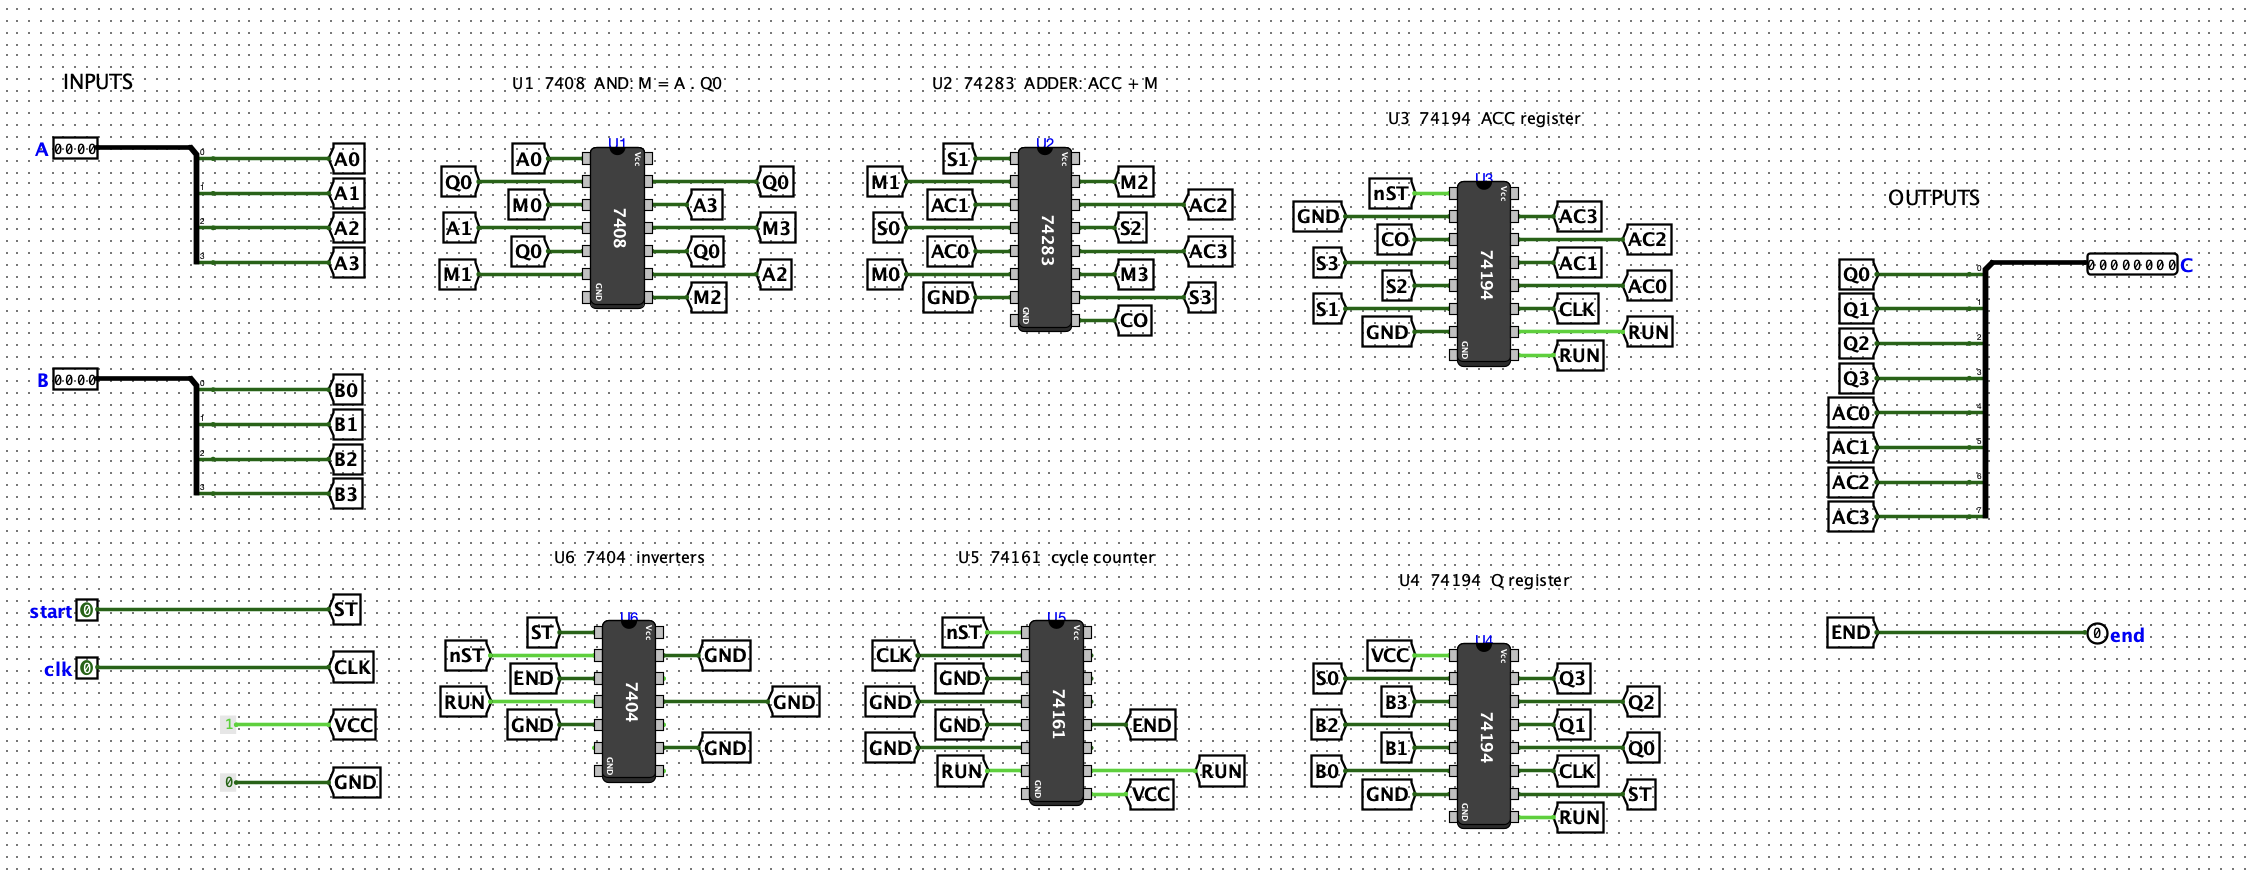
\includegraphics[width=1\textwidth]{figs/multiplier.png}
}
}


\subsubsection*{مدار \lr{main}}

{
\centering{
  
\includegraphics[width=0.9\textwidth]{figs/main.png}
}
}



\end{document}
